\section{Tunnelling, Time-Dependent Perturbation Theory}

\subsection{Review of WKB}
We can solve tunnelling for arbitrary potentials $U(x)$ using WKB. We will derive this formula and discuss when it is justified. 

\begin{figure}[htbp]
    \centering
    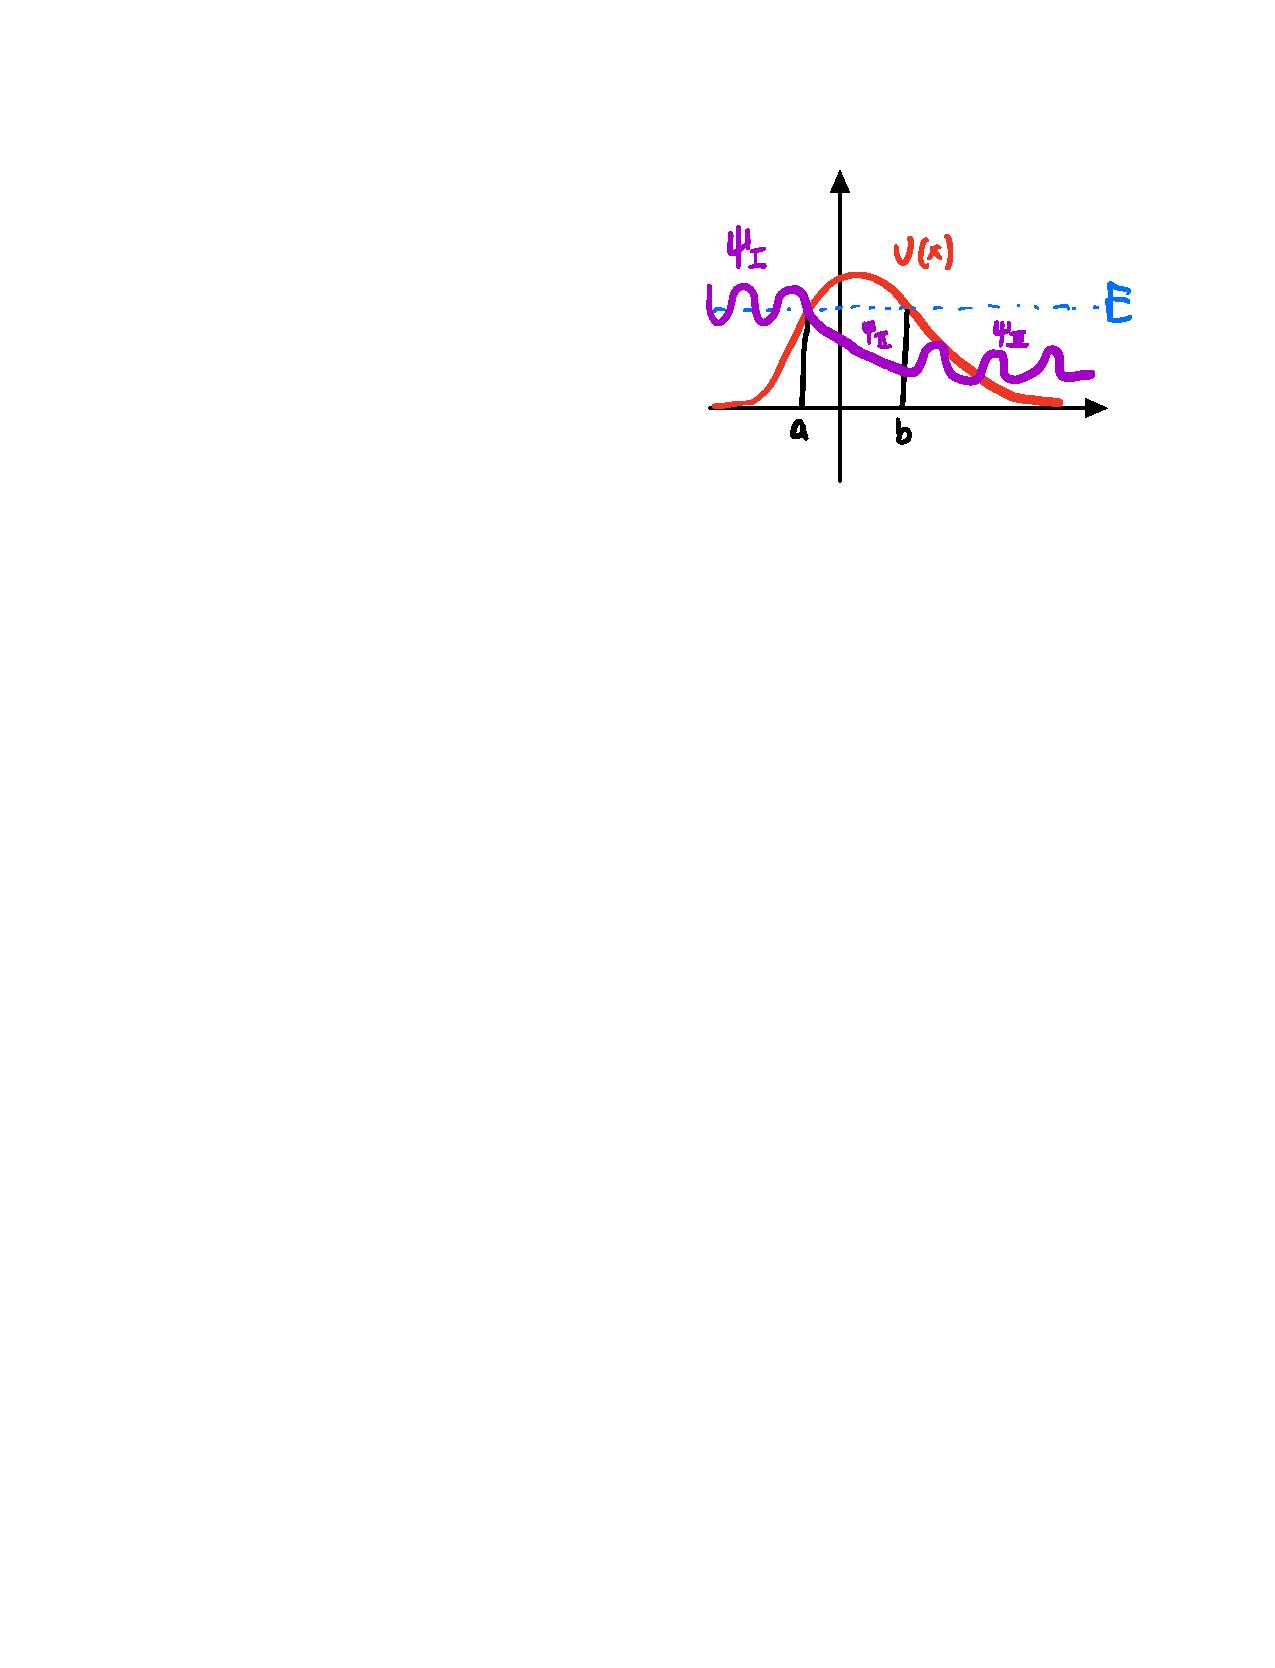
\includegraphics[]{Images/fig-WKBtunnelling.pdf}
    
    \caption{Using WKB to study quantum mechanical tunnelling. We have a particle incoming from the left in a classically allowed region, where the wavefunction is sinusoidal ($\psi_{I}$). In the classically forbidden region, the amplitude of the wavefunction exponentially decays ($\psi_{II}$). Finally, after the barrier, the wavefunction is again sinusoidal ($\psi_{III}$), but the amplitude is down exponentially from the wavefunction in the first region. We can use WKB and the connection formulas to obtain the approximate wavefunctions in each region, and find the transmission coefficient.}
    \label{fig-WKBtunnelling}
\end{figure}

Previously, we discussed getting the energy for an arbitrary potential:

\begin{figure}[htbp]
    \centering
    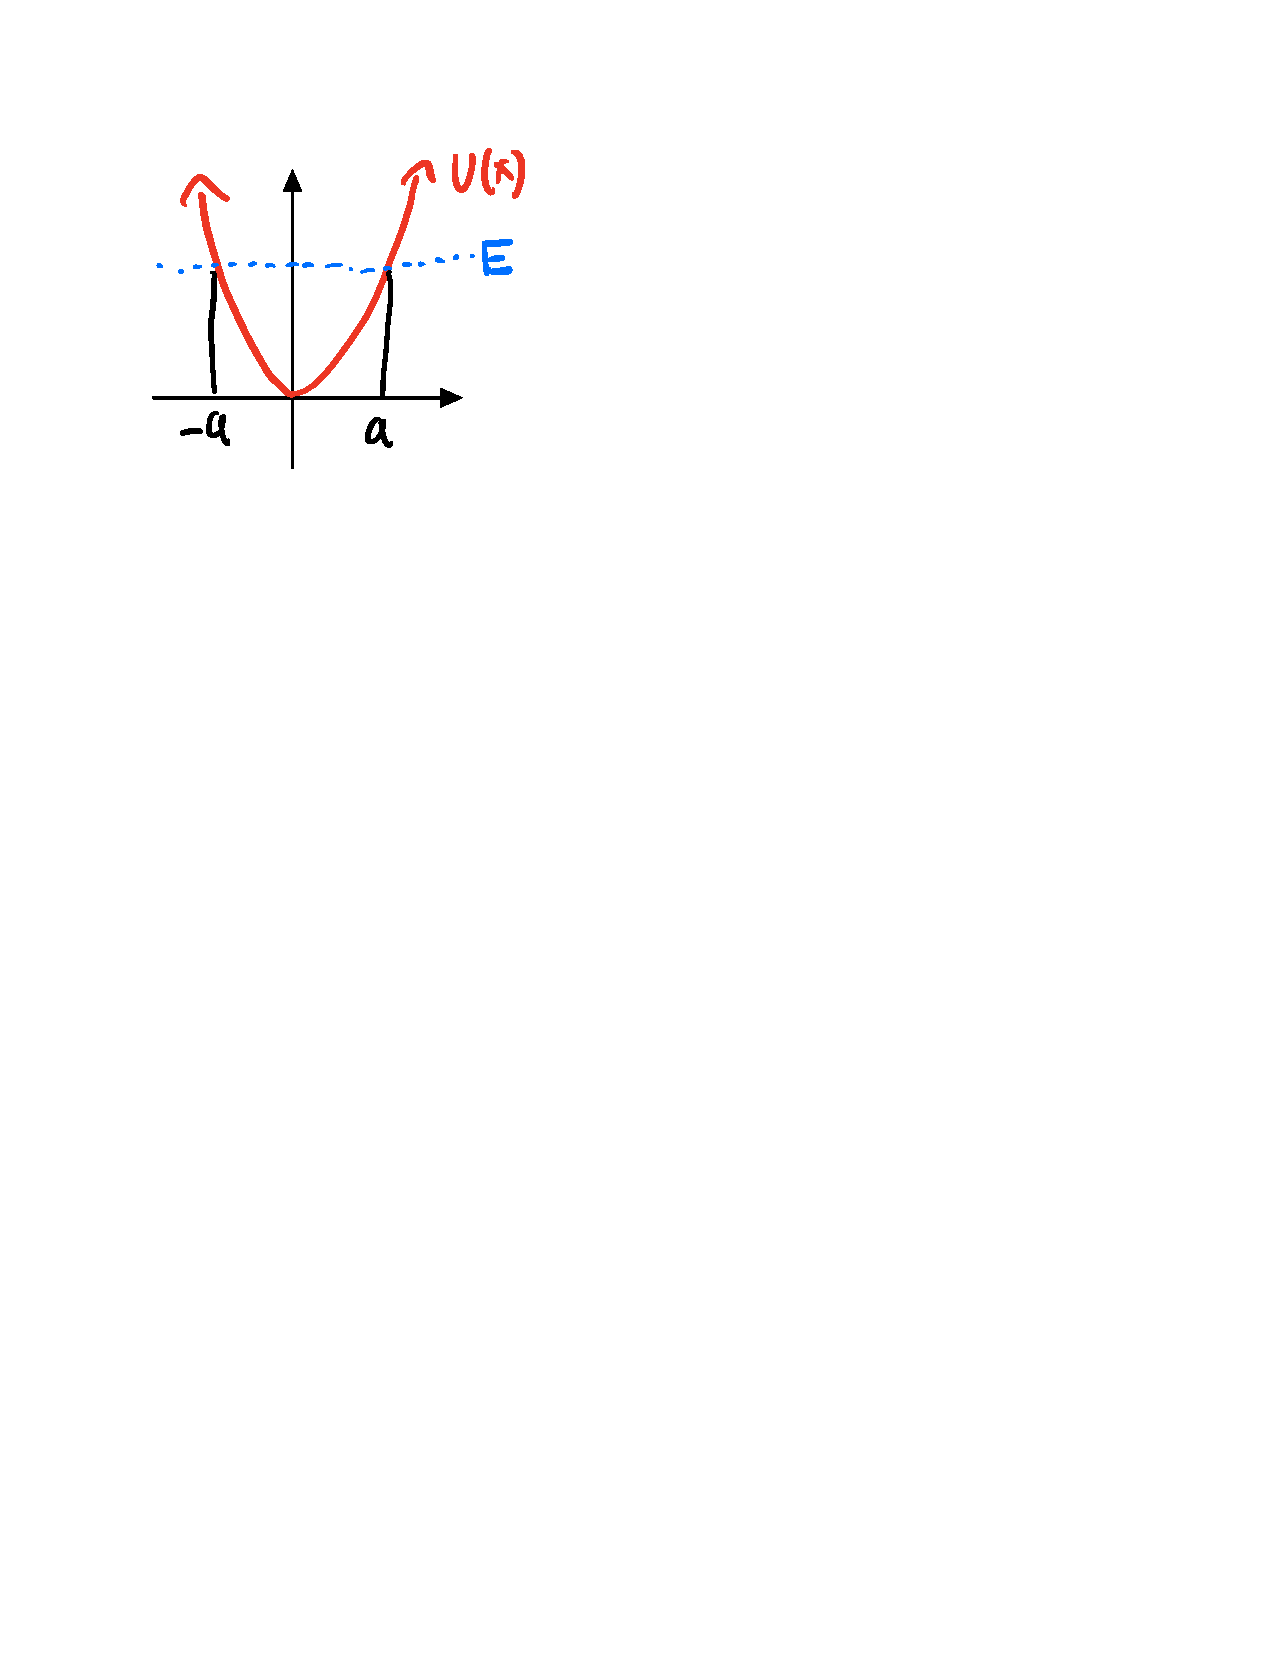
\includegraphics[scale=0.8]{Images/fig-WKBenergies.pdf}
    
    \caption{Last time, we found the energies of the Harmonic oscillator (quadratic potential) using the WKB approximation.}
    \label{fig-energyWKB}
\end{figure}


We considered carrying out the integral (classically):
\begin{equation}
    \int_{-a}^a \frac{pdx}{\hbar} = \pi(n + \frac{1}{2})
\end{equation}
Where $p^2/2m = E - U(x)$.

If we compare Fig. \ref{fig-tunnelling} and Fig. \ref{fig-energyWKB}, we can see in a hand-wavey way that we ``flip'' the potential between the two cases.

\subsection{Tunneling Derivation}
Using the WKB approximation, we can write the wavefunction in the three regions of Fig. \ref{fig-tunnelling} as:
\begin{equation}
    \psi_{III} = \frac{C}{\sqrt{p}} e^{i\int_b^x \frac{p(x')dx'}{\hbar} + \frac{i\pi}{4}}
\end{equation}
\begin{equation}
    \psi_{II} = \frac{C}{\sqrt{p}}e^{+\int_x^{b}\frac{pdx'}{\hbar}} + \frac{C}{\sqrt{p}}e^{-\int_x^b \frac{p(x')dx'}{\hbar}} = \frac{C}{\sqrt{p}}e^{\frac{p dx'}{\hbar}}
\end{equation}
We discard the second term in the above $\psi_{II}$ which is exponentially small, as the WKB approximation cannot recover exponentially small pieces. We are using the connection formula we derived previously to conclude that the $C$s are the same in the two formulas. We then write:
\begin{equation}
    \psi_{II} = \frac{C}{\sqrt{p}}e^{+\int_a^b\frac{pdx'}{\hbar}}e^{-\int_a^x \frac{pdx'}{\hbar}} = Ce^{\int_a^b \frac{pdx'}{\hbar}}\frac{1}{\sqrt{p}}e^{-\int_a^x \frac{pdx'}{\hbar}}
\end{equation}
The minus sign in the exponential means that the incoming particle from the right exponentially decays in the $II$ region. In $I, III$ the wavefunctions will be oscillatory. The question then becomes how much does the amplitude decrease between the two regions. Writing down the wavefunction in region $I$:
\begin{equation}
    \psi_I = \frac{D}{\sqrt{p}}\left[e^{+i\int_a^x \frac{p(x')dx'}{\hbar} + \frac{i\pi}{4}} + e^{-i\int_a^x \frac{p(x')dx'}{\hbar} - \frac{i\pi}{4}}\right]
\end{equation}
The transmission coefficient is:
\begin{equation}
    T = \frac{\abs{C}^2}{\abs{D}^2} = e^{-2\int_a^b \frac{p(x')dx'}{\hbar}}
\end{equation}
The reflection coefficient cannot actually be restored/computed using the WKB calculation, because we have discarded the exponentially supressed part in $\psi_{II}$. However, we can in general say $R = 1 - T$. 

When is the above formula is justified? When we have a highly excited state. Mathematically, this is when:
\begin{equation}
    \int_a^b \frac{pdx'}{\hbar} \gg 1.
\end{equation}
or when:
\begin{equation}
    T \ll 1.
\end{equation}
I.e. the transmission is very small. The WKB approximation fails when $E \approx U$, i.e. when the energy of the incoming particle is close to the height of the potential well. In this case there would not be a significant decay of the wavefunction inside of the well.

We will explore this on Q3 of the HW3.

\subsection{Motivating Time-Dependent Perturbation Theory}
Up until this point, we had a time-independent Hamiltonian $H$, and we could express the time evolution of an arbitrary state $\psi(x, t)$ as:
\begin{equation}
    \psi(x, t) = \sum_n c_n \psi_n e^{-i\frac{E_n t}{\hbar}}
\end{equation}
and if we had an eigenstate, there would be no time-evolution whatsoever. Of course this is not what happens in real life; a highly excited hydrogen atom state does not stay in this same state forever. We require the study of time-dependent perturbations for this, so let us begin.

\subsection{Developing Time-Dependent Perturbation Theory}
We consider a two-level system with Hamiltonian $H^{(0)}$ with eigenstates $\ket{\psi_a}, \ket{\psi_b}$ such that:
\begin{equation}
    H^{(0)}\ket{\psi_a} = E_a\ket{\psi_a}, \quad H^{(0)}\ket{\psi_b} = E_b\ket{\psi_b}
\end{equation}
\begin{equation}
    \bra{\psi_a}{\psi_b} = \delta_{ab}
\end{equation}
and the evolution of a general state was given by:
\begin{equation}\label{eq-psit}
    \ket{\psi(t)} = c_a\ket{\psi_a}e^{-i\frac{E_a t}{\hbar}}  + c_b\ket{\psi_b}e^{-i\frac{E_b t}{\hbar}}.
\end{equation}
Now we consider some time-dependent perturbation $H'(t)$, and we ask what the transition probability is. Let us try to figure it out. The total Hamiltonian is:
\begin{equation}
    H = H^{(0)} + H'(t)
\end{equation}
so we can write down the Schrodinger equation:
\begin{equation}
    i\hbar \dpd{\ket{\psi}}{t} = H\ket{\psi}
\end{equation}
Therefore evaluating the LHS for $\ket{\psi(t)}$ as in Eq. \eqref{eq-psit} we have:
\begin{equation}
    \begin{split}
        &i\hbar \dpd{\ket{\psi(t)}}{t}
        \\ &= i\hbar\dot{c}_a\ket{\psi_a}e^{-i\frac{E_at}{\hbar}} + i\hbar c_a\left(-i\frac{E_a}{\hbar}\right)\ket{\psi_a}e^{-i\frac{E_a t}{\hbar}}
        \\ &+ i\hbar\dot{c}_b\ket{\psi_b}e^{-i\frac{E_bt}{\hbar}} + i\hbar c_b\left(-i\frac{E_b}{\hbar}\right)\ket{\psi_b}e^{-i\frac{E_b t}{\hbar}}
    \end{split}
\end{equation}
Evaluating the RHS we then have:
\begin{equation}
    \begin{split}
        &H\ket{\psi(t)} 
        \\ &= c_aE_a\ket{\psi_a}e^{-i\frac{E_at}{\hbar}} + c_bE_b\ket{\psi_b}e^{-i\frac{E_b t}{\hbar}}
        \\ &+ H'c_a\ket{\psi_a}e^{-i\frac{E_a t}{\hbar}} + H'c_b\ket{\psi_b}e^{-i\frac{E_b t}{\hbar}}
    \end{split}
\end{equation}
We can cancel out the terms of the above that come from the SE with the time-independent Hamiltonian $H$ (i.e. the second column of terms on the LHS and the first row of terms on the RHS). Now, multiplying both sides on the right with $\bra{\psi_a}$ and using orthogonality, we find:
\begin{equation}
    i\hbar \dot{c}_a = c_a\bra{\psi_a}H'(t)\ket{\psi_a} + \bra{\psi_a}H'(t)\ket{\psi_b}c_b e^{-i\frac{E_b - E_a}{\hbar}t}
\end{equation}
and analogously for $\bra{\psi_b}$:
\begin{equation}
    i\hbar \dot{c}_b = c_b\bra{\psi_b}H'(t)\ket{\psi_b} + \bra{\psi_b}H'(t)\ket{\psi_a}c_a e^{-i\frac{E_a - E_b}{\hbar}t}
\end{equation}
So far we have not done anything approximate; everything has been analytic. We now make our first simplification; we consider:
\begin{equation}
    \bra{\psi_a}H'(t)\ket{\psi_a} = \bra{\psi_b}H'(t)\ket{\psi_b} = 0.
\end{equation}
as we are only interested in the transitions between the states (but it is trivial to generalize this to the case where the above are nonzero). With this our formulas simplify:
\begin{equation}
    \begin{split}
        \dot{c}_a &= \frac{-i}{\hbar}c_b \bra{\psi_a}H'(t)\ket{\psi_b}e^{-i\omega t}
        \\  \dot{c}_b &= \frac{-i}{\hbar}c_a\bra{\psi_b}H'(t)\ket{\psi_a}e^{i\omega t}
    \end{split}
\end{equation}
where $\omega = \frac{E_b - E_a}{\hbar}$. But note we have not made any assumptions about the weakness of our potentials, or anything like that. Note that solving the above formula is in general quite difficult to solve; so we will develop PT techniques for it.